\documentclass[12pt,a4paper]{scrartcl}

\usepackage{ucs}
\usepackage[utf8x]{inputenc}
\usepackage[T1]{fontenc}
\usepackage[ngerman]{babel}
\usepackage{graphicx}
\usepackage{amsmath,amssymb,amstext}
\usepackage{subscript}

\usepackage{lastpage}

\inputencoding{utf8}

\title{Modulation 3 \\PAM PCM}
\date{\today{}}
\author{Rafael Haigermoser}
%Kopf und Fuszeile
\usepackage{scrlayer-scrpage}
\pagestyle{scrheadings}
\clearpairofpagestyles

\pagenumbering{arabic}
 %graph
\usepackage{pgfplots}
\usepackage{pgfplotstable}
\usepackage{booktabs}
\usepackage{array}
\usepackage{colortbl}

\pgfplotstableset{% global config, for example in the preamble
  every head row/.style={before row=\toprule,after row=\midrule},
  every last row/.style={after row=\bottomrule},
  fixed,precision=2,
}


\ihead{Laborprotokoll}
\chead{}
\ohead{Modulation 3\\PAM PCM}
\ifoot{Rafael Haigermoser}
\cfoot{HTBLuVA-Salzburg}
\ofoot{\pagemark / \pageref{LastPage} }

\begin{document}

    \maketitle
    \newpage
    \tableofcontents
    \newpage
   
    \section{Einleitung}
    \label{sec:einleitung}
        Die Pulsamplitudenmodulation und wird verwendet, um Signale über kurze Strecken zu übertragen, da sie besonders einfach zu erzeugen ist. Dabei ist das Abtasttheorem zu beachten, weil sonst Aliasing auftritt. Außerdem werden Zeitmultiplexverfahren behandelt, mit welchen verschiedene Signale über die gleiche Leitung gleichzeitig übertragen werden können.
    \section{Inventarliste}
    \label{sec:inventarliste}
    \begin{tabular}{rlr}
      Stück & Gerätebezeichnung \\
             1 & Keysight Digital Storage Oscilloscope  \\
             1 & HPS-Modulation-Board       \\
             4 & Koaxialmessstrippen \\
    \end{tabular}
    
    
    \section{Übungsdurchführung}
    \label{sec-übungsdurchfürung}
        \subsection{Erzeugung eines pulsamplitudenmodulierten Signals}
        \label{sub-sec-pulsamplitudenmoduliertes-signal}
        In Abbildung \ref{fig:pulsamplitudenmoduliertes-signal} wird wie auf Seite 148 der Angaben ein Sinussignal pulsamplitudenmoduliert.
       
U\textsubscript{s}  f= 8kHz der Impuls dauert aber nur ca. 15us. \\
        U\textsubscript{inf} f=1kHz \^{U}=1,5V ein Sinussignal\\
        U\textsubscript{PAM} das pulsamplitudenmodulierte Signal
        

               
    \begin{figure}[htbp]
    \begin{minipage}{1\textwidth}
         \centering
         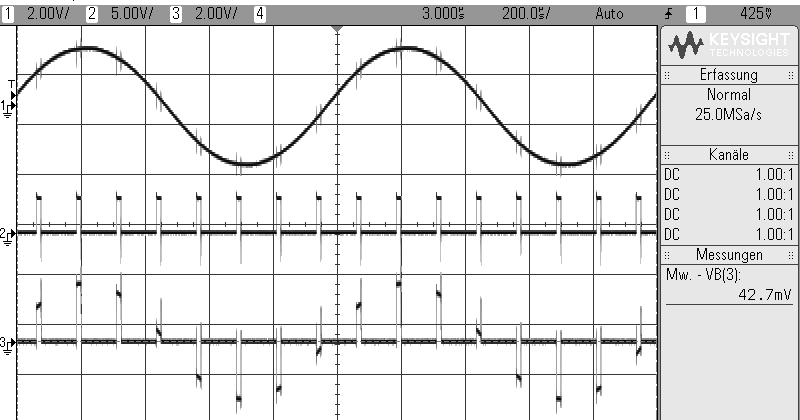
\includegraphics[width=1\textwidth]{scope_0}
         \caption{U\textsubscript{s}, U\textsubscript{inf}, U\textsubscript{PAM},}
   
          \label{fig:pulsamplitudenmoduliertes-signal}
    \end{minipage}
    \end{figure}
    \newpage
    Frage Seite 150: Wie ist die Schaltung in Abb. 6.2.3 zu erweitern, damit ein unipolares PAM-Signal entsteht? Ergänzen Sie die Schaltung und zeichnen Sie die Ausgangsspannung in das Diagramm Abb. 6.2.5 ein.\\ Antwort: Die Schaltung wird durch eine Diode erweitert, das Ausgangssignal ist in Abb. \ref{fig:pulsamplitudenmoduliertes-signal-gleichgerichtet} zu sehen.
    
    \begin{figure}[htbp]
    \begin{minipage}{1\textwidth}
         \centering
         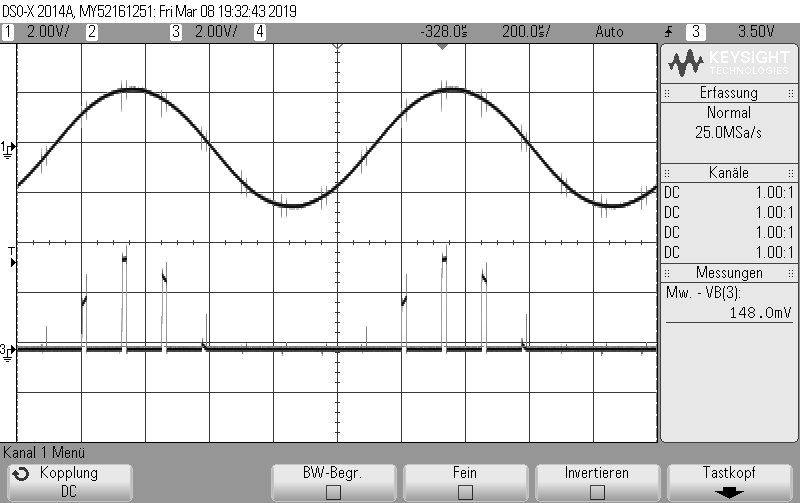
\includegraphics[width=1\textwidth]{scope_1}
         \caption{U\textsubscript{s}, U    \textsubscript{PAM},}
   
          \label{fig:pulsamplitudenmoduliertes-signal-gleichgerichtet}
    \end{minipage}
    \end{figure}
    \newpage
    
    
    \subsection{Frequenzspektrum des pulsamplitudenmodulierten Signals}
        \label{sub-sec-frequenz-pulsamplitudenmoduliertes-signal}
        Fragen Seite 152:\\
         1. Bei welcher Frequenz ist das erste Minimum in der Amplitude der Spektrallinien zu beobachten?\\
          Bei 67kHz, wie in Abb. \ref{fig:scope_6} zu sehen ist.\\
           \begin{figure}[htbp]
    \begin{minipage}{1\textwidth}
         \centering
         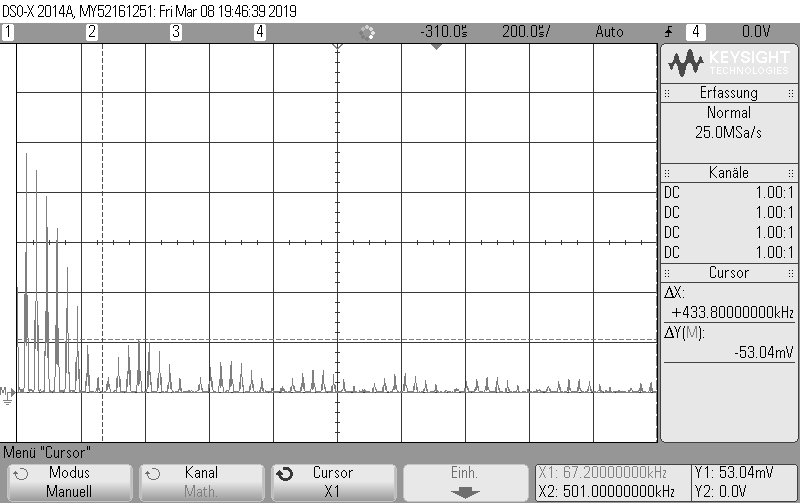
\includegraphics[width=1\textwidth]{scope_6}
         \caption{Frequenzspektrum des zuvor erzeugten PAMs}
   
          \label{fig:scope_6}
    \end{minipage}
    \end{figure}\\
    
          2. Stimmt das meßtechnisch ermittelte Minimum mit dem rechnerischen Wert überein?\\
          \begin{equation*}
f=\frac{1}{\tau}		    
	\end{equation*}
       
       Ja, es ist 66,\.{6} kHz.
       \newpage
       3. In welchem Frequenzabstand folgen die Spektrallinien, wenn nur der Abtastimpuls analysiert wird?\\
       Sie folgen im Frequenzabstand von 8.2kHz, wie es in Abb. \ref{fig:scope_11} zu sehen ist. \\
       \begin{figure}[htbp]
    \begin{minipage}{0.72\textwidth}
     \centering
      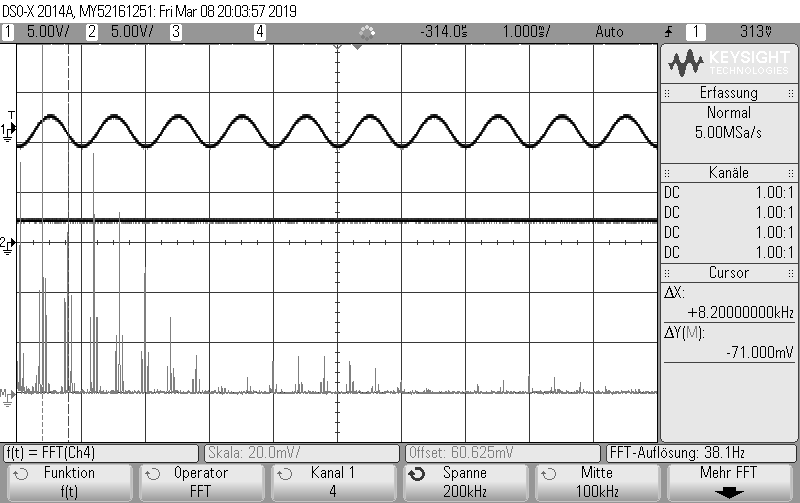
\includegraphics[width=1\textwidth]{scope_11}
      \caption{Frequensspektrum eines PAM-Signals}
      \label{fig:scope_11}
    \end{minipage}\hfill
  \end{figure} 
  
       4. Wie unterscheidet sich das Spektrum einer unipolaren von dem einer bipolaren PAM?\\
       Im Abstand der Abtastfrequenz sind auch Linien zu sehen, Abb. \ref{fig:scope_12} bipolar und \ref{fig:scope_13}unipolar.
       
    
    \begin{figure}[htbp]
    \begin{minipage}{0.48\textwidth}
     \centering
      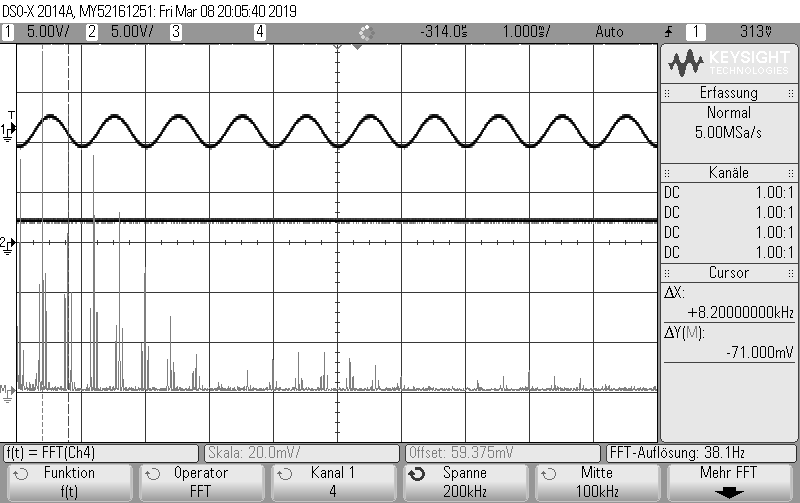
\includegraphics[width=1\textwidth]{scope_12}
      \caption{Frequenzsspektrum des PAM bipolar}
      \label{fig:scope_12}
    \end{minipage}\hfill
    \begin{minipage}{0.48\textwidth}
     \centering
      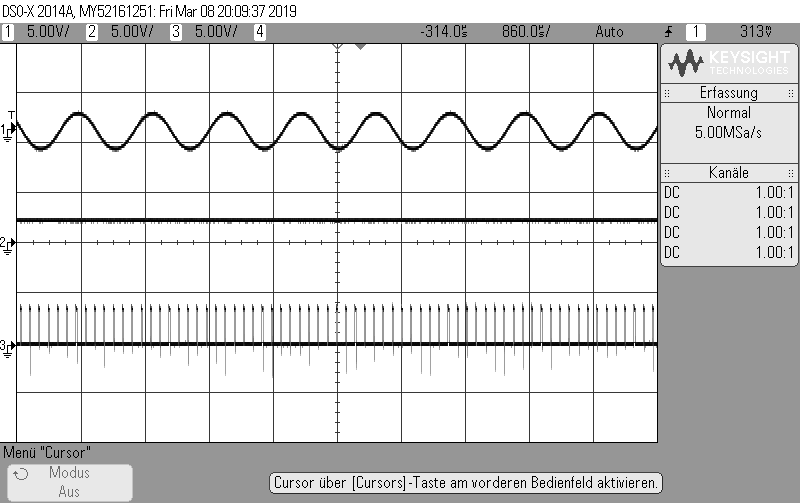
\includegraphics[width=1\textwidth]{scope_13}
      \caption{Freqeunzsspektrum des PAM unipolar}
      \label{fig:scope_13}
    \end{minipage}
  \end{figure} 
  \newpage
  5. Wie kann ein PAM-Signal demoduliert werden?\\   Es kann mit einem Tiefpassfilter demoduliert werden.   
  \\Arbeitsauftrag Seite 153:\\
 Bei Abb. \ref{fig:scope_8} U\textsubscript{inf}:  1kHz \^{U}=2V
        U\textsubscript{DC}=0V
        U\textsubscript{S} 8 kHz TTL-Pegel
        
  \begin{figure}[htbp]
    \begin{minipage}{0.8\textwidth}
     \centering
      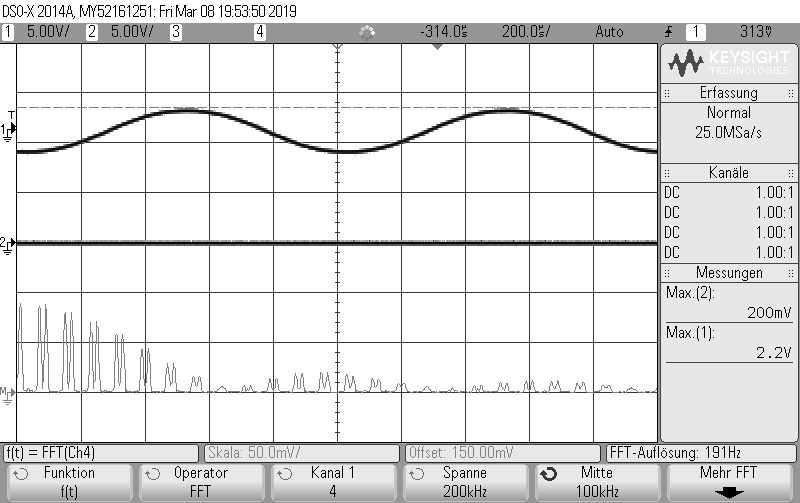
\includegraphics[width=1\textwidth]{scope_8}
      \caption{Frequenzsspektrum eines PAM-Signals}
      \label{fig:scope_8}
    \end{minipage}\hfill
  \end{figure}
  
  \newpage
  Bei Abb. \ref{fig:scope_9} U\textsubscript{inf}:  1kHz \^{U}=2V
        U\textsubscript{DC}=0V
        U\textsubscript{S} 8 kHz TTL-Pegel
        
  \begin{figure}[htbp]
    \begin{minipage}{0.72\textwidth}
     \centering
      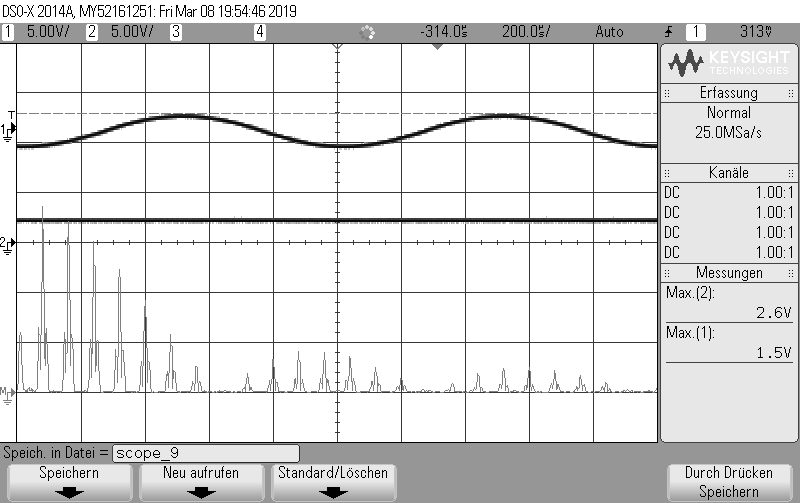
\includegraphics[width=1\textwidth]{scope_9}
      \caption{Frequenzsspektrum eines PAM-Signals}
      \label{fig:scope_9}
    \end{minipage}\hfill
  \end{figure}
  
  
  Bei Abb. \ref{fig:scope_10} U\textsubscript{inf}:  1kHz \^{U}=2V
        U\textsubscript{DC}=0V
        U\textsubscript{S} 8 kHz TTL-Pegel
        
  \begin{figure}[htbp]
    \begin{minipage}{0.72\textwidth}
     \centering
      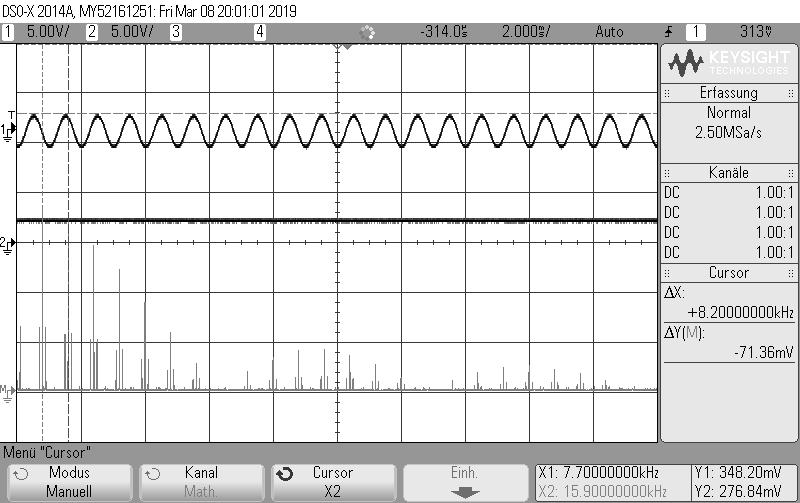
\includegraphics[width=1\textwidth]{scope_10}
      \caption{Frequenzsspektrum eines PAM-Signals}
      \label{fig:scope_10}
    \end{minipage}\hfill
  \end{figure} 
  \newpage
       
       
    \subsection{Überprüfung des Abtasttheorems}
    \label{sub-sec-abtasttheorem}
    Frage: 
    In welchen Fällen kann das Informationssignal nicht mehr durch einen Tiefpass f\textsubscript{g}=3,4kHz aus dem PAM-Signa herusgefiltert werden?
    
    Arbeitsauftrag Seite 158:
    Bei dieser Aufgabe wird ein unipolares PAM erzeugt, und bei unterschiedlichen Informations- und Abtastfrequenzen untersucht. Frequenzspektrum wurde bei den vorgegebenen Frequensspekteren gemessen.\\
     \begin{figure}[htbp]
    \begin{minipage}{0.48\textwidth}
     \centering
      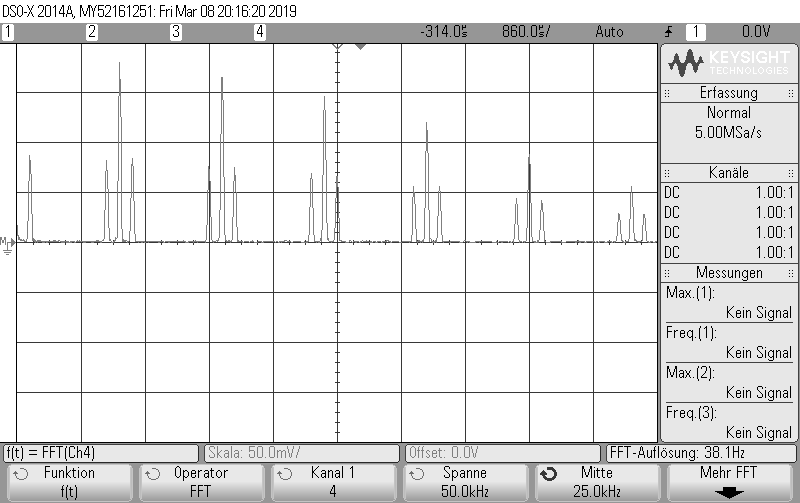
\includegraphics[width=1\textwidth]{scope_15}
      \caption{}
      \label{fig:scope_15}
    \end{minipage}\hfill
    \begin{minipage}{0.48\textwidth}
     \centering
      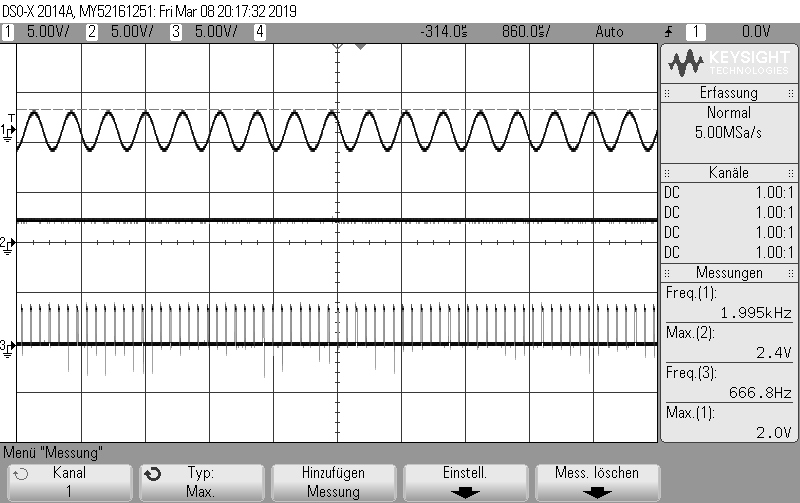
\includegraphics[width=1\textwidth]{scope_16}
      \caption{}
      \label{fig:scope_16}
    \end{minipage}
  \end{figure} 
  Bei Abb. \ref{fig:scope_15} und \ref{fig:scope_16} U\textsubscript{inf}:  1kHz \^{U}=2V
        U\textsubscript{DC}=2,5V
        U\textsubscript{S} 8 kHz TTL-Pegel\\
     \begin{figure}[htbp]
    \begin{minipage}{0.48\textwidth}
     \centering
      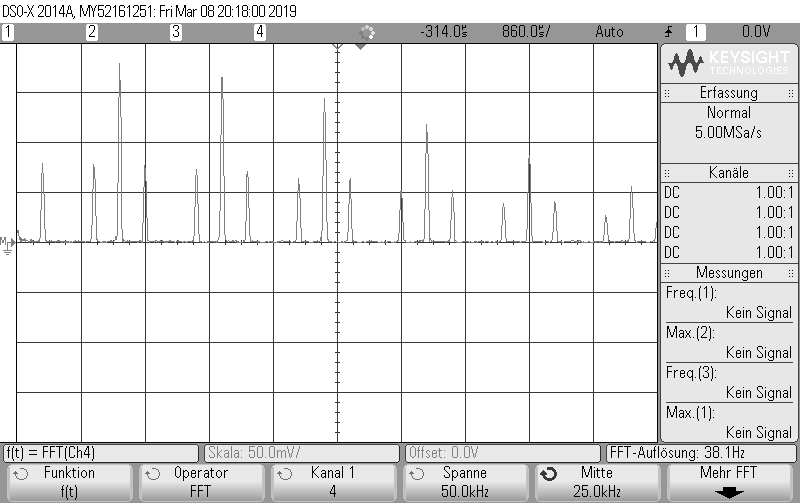
\includegraphics[width=1\textwidth]{scope_17}
      \caption{}
      \label{fig:scope_17}
    \end{minipage}\hfill
    \begin{minipage}{0.48\textwidth}
     \centering
      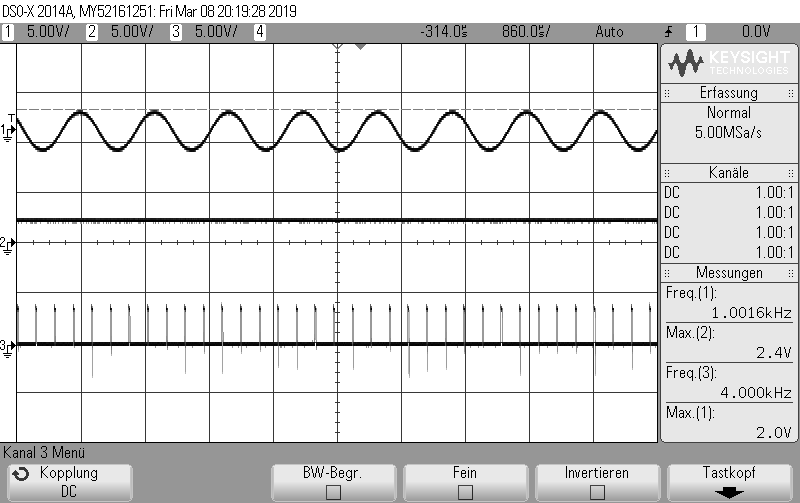
\includegraphics[width=1\textwidth]{scope_18}
      \caption{}
      \label{fig:scope_18}
    \end{minipage}
  \end{figure} 
   Bei Abb. \ref{fig:scope_17} und \ref{fig:scope_18} U\textsubscript{inf}:  2kHz \^{U}=2V
        U\textsubscript{DC}=2,5V
        U\textsubscript{S} 8 kHz TTL-Pegel
        \newpage
     \begin{figure}[htbp]
    \begin{minipage}{0.48\textwidth}
     \centering
      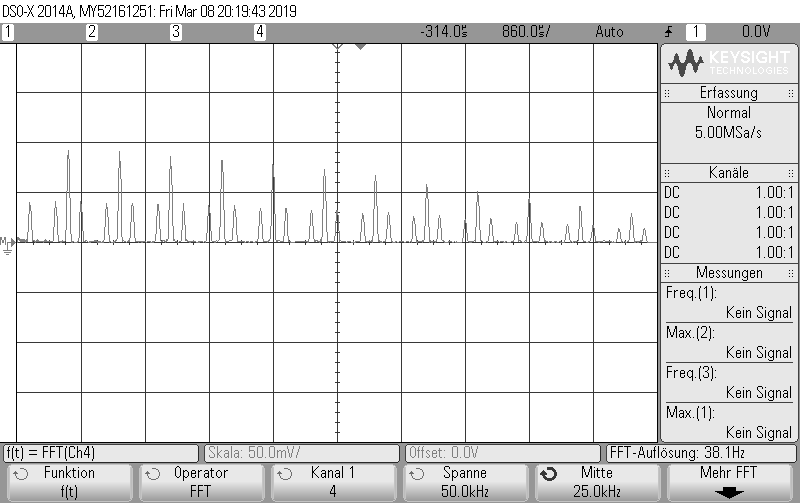
\includegraphics[width=1\textwidth]{scope_19}
      \caption{}
      \label{fig:scope_19}
    \end{minipage}\hfill
    \begin{minipage}{0.48\textwidth}
     \centering
      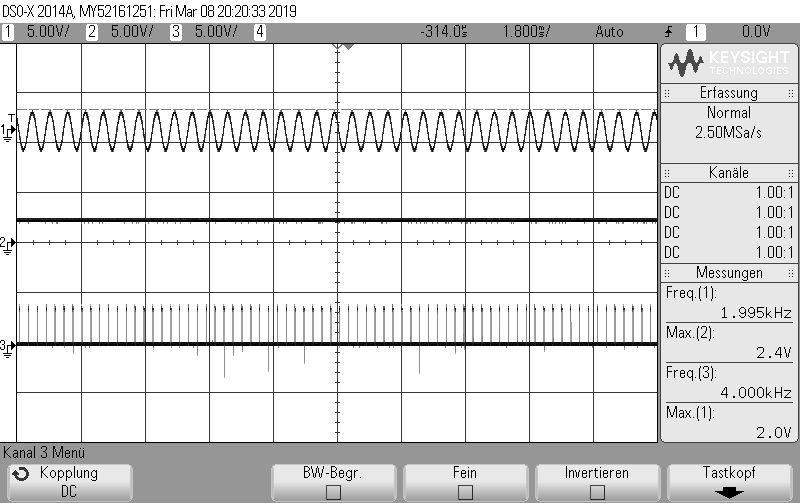
\includegraphics[width=1\textwidth]{scope_20}
      \caption{}
      \label{fig:scope_20}
    \end{minipage}
  \end{figure} 
   Bei Abb. \ref{fig:scope_19} und \ref{fig:scope_20} U\textsubscript{inf}:  1kHz \^{U}=2V
        U\textsubscript{DC}=2,5V
        U\textsubscript{S} 4 kHz TTL-Pegel \\
     \begin{figure}[htbp]
    \begin{minipage}{0.48\textwidth}
     \centering
      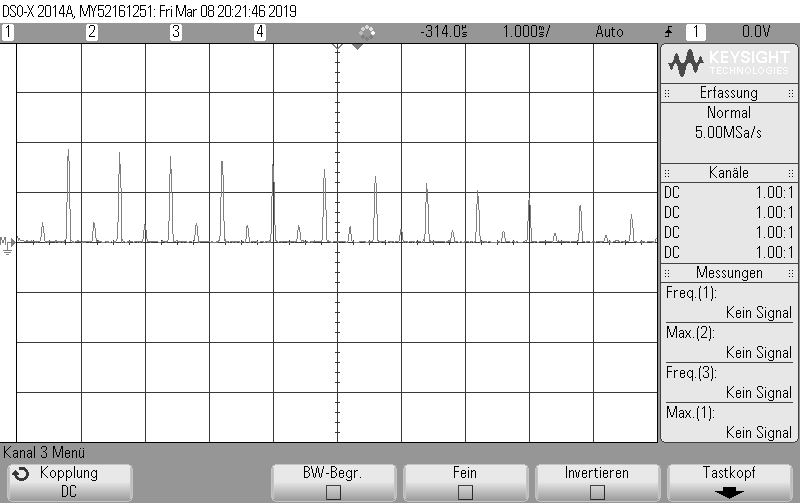
\includegraphics[width=1\textwidth]{scope_21}
      \caption{}
      \label{fig:scope_21}
    \end{minipage}\hfill
    \begin{minipage}{0.48\textwidth}
     \centering
      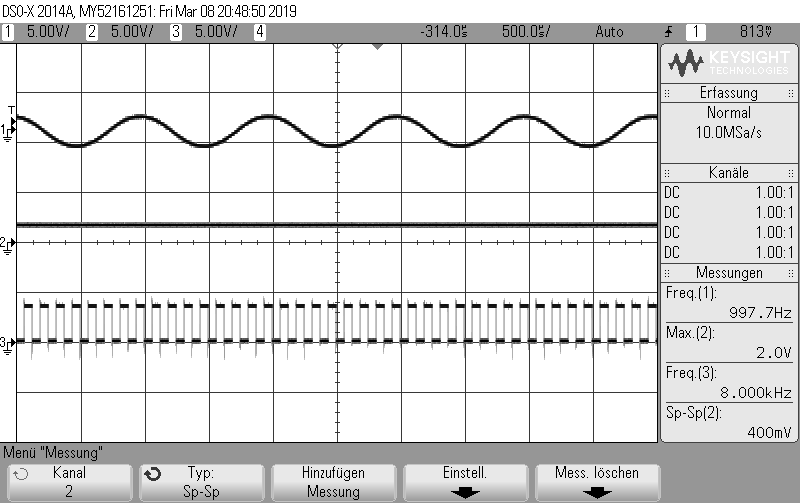
\includegraphics[width=1\textwidth]{scope_22}
      \caption{}
      \label{fig:scope_22}
    \end{minipage}
  \end{figure} 
   Bei Abb. \ref{fig:scope_21} und \ref{fig:scope_22} U\textsubscript{inf}:  1kHz \^{U}=2V
        U\textsubscript{DC}=2,5V
        U\textsubscript{S} 8 kHz TTL-Pegel
        \newpage
  \subsection{Zeitmultiplexverfahren}
  \label{sub-sec-zeitmultiplexverfahren}
  Fragen:
  1. Handelt es sich bei der Spannung U\textsubscript{PAM} um  eine unipolare oder um eine bipolare PM?
  Es ist bipolar siehe Abb. \ref{fig:scope_23}.
    \begin{figure}[htbp]
    \begin{minipage}{1\textwidth}
         \centering
         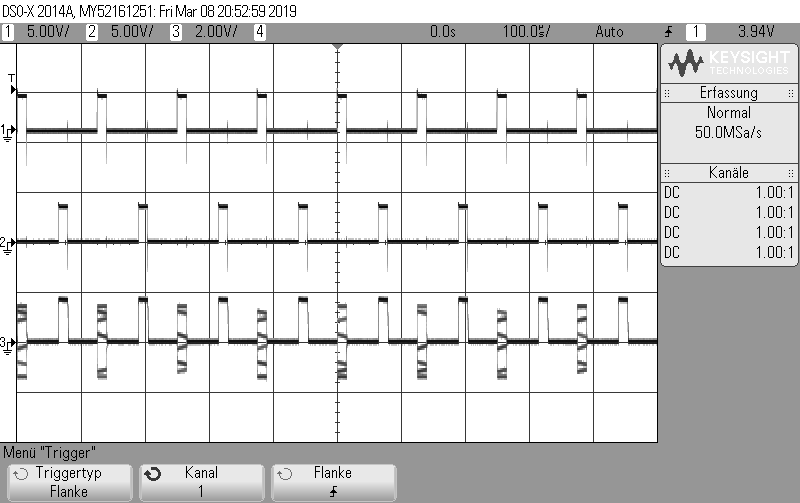
\includegraphics[width=1\textwidth]{scope_23}
         \caption{U\textsubscript{PAM} ist die unterste Spnnung}
   
          \label{fig:scope_23}
    \end{minipage}
    \end{figure}\\
    2.Wieviele Kanäle könnte man theoretisch unter Beibehaltung der 8-kHz-Abtastfrequenz bei 15us Impulsbreite übertragen?\\
    Man könnte 8 Kanäle übertragen.
    
    \begin{equation}
		\frac{1}{8kHz} = 125us
	\end{equation}
	\begin{equation}
		\frac{125us}{15us} =8,33
	\end{equation}
	3. Weshalb wird die PAM-Multiplextechnik nicht auf Übertragungsstrecken verwendet?\\
Sie hat wenig Energie und wird deswegen leicht gestört.
\newpage
Versuchsaufbau Seite 162 mit den Werten:\\
U\textsubscript{inf 1}:  1kHz \^{U}=1,5V\\
U\textsubscript{inf 2}:  U = +2V\\
U\textsubscript{Sync}= f= 8kHz TTL-Pegel
      \begin{figure}[htbp]
    \begin{minipage}{0.48\textwidth}
     \centering
      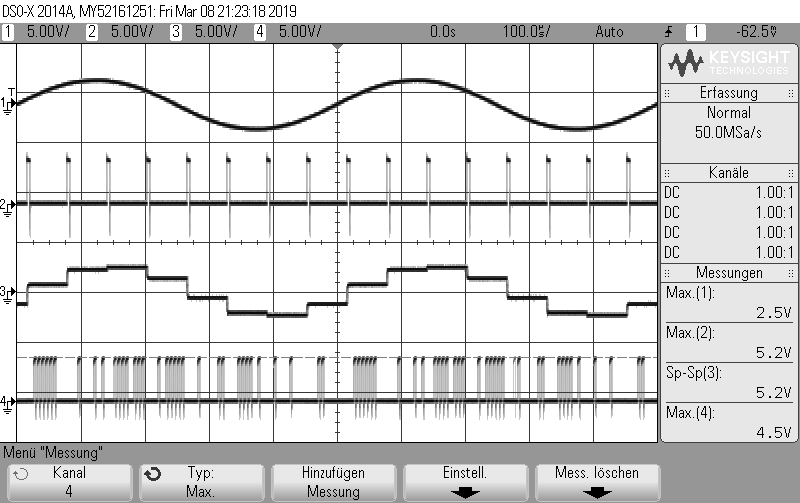
\includegraphics[width=1\textwidth]{scope_25}
      \caption{}
      \label{fig:scope_25}
    \end{minipage}\hfill
    \begin{minipage}{0.48\textwidth}
     \centering
      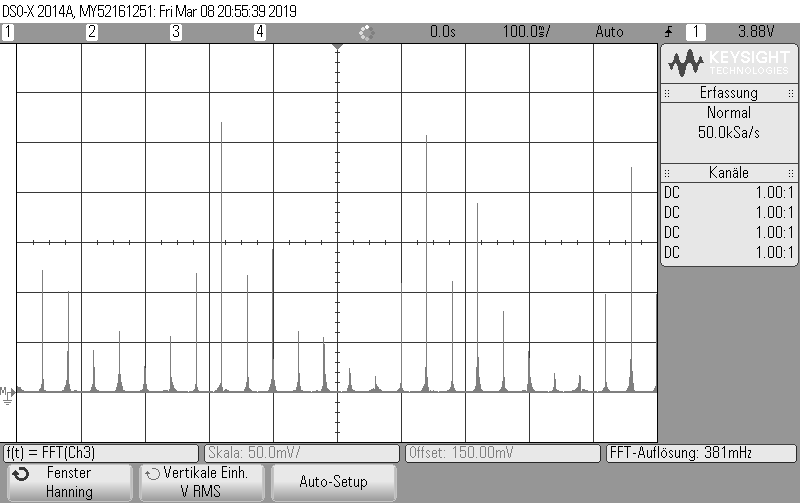
\includegraphics[width=1\textwidth]{scope_24}
      \caption{}
      \label{fig:scope_24}
    \end{minipage}
  \end{figure} \\
  Wiederholungsfragen:
  1. Wie groß sollte die Bandbreite eines Übertragungssystems sein, wenn die Pulsbreite 15us beträgt?
  Sie beträgt 66kHz
  \begin{equation}
		\frac{1}{15us} =66kHz
    \end{equation}\\
    2. Mit welcher Abtastfrequenz muss ein Signal abgetastet werden, dessen höchste Frequenz bei 15kHz liegen?\\
    Mit mindestens 30kHz, damit das Abtastthorem eingehalten wird.\\
    3. Wiso muss vor der Abtastung eine Frequenzbandbegrenzung erfolgen?\\
    Weil sonst Aliasing auftreten kann.\\
    4. Welche Pulsfolgenfrequenz hat ein System, das mit 8kHz abgetastet wird und 32 Kanäle hat?\\
    Es hat eine Pulsfolgenfrequenz von 256kHz, siehe Rechnung \ref{eq:4.1} bis \ref{eq:4.3}
    \begin{equation}
    	\label{eq:4.1}
		\frac{1}{8kHz} = 125us
    \end{equation}\\
    \begin{equation}
		\frac{125us}{32} = 3,9us
    \end{equation}\\
    \begin{equation}
    	\label{eq:4.3}
		\frac{1}{3,9us} = 256kHz
    \end{equation}\\
  \newpage
  \subsection{Pulscodemodulation}
  \label{sub-sec-pulscodemodulation}
Es wird die Kennlinie des AD-Wandlers aufgenommen.\\
  \pgfplotstableread{pulscodmodulation.txt}\loadedtable
\pgfplotstabletranspose[]{\transposetable}{\loadedtable}  
\pgfplotstabletypeset[string type]\loadedtable

	\begin{tikzpicture}
		\begin{axis}[
		title={Kennlinie des A/D-Wandlers},
					xlabel={Spannung (V)},
					ylabel={Nummer des Quantisierungsintervalls}]
			\addplot table[x=Spannung, y=Dezimalwert] {pulscodmodulation.txt};
			
		\end{axis}

	\end{tikzpicture}
	
	\newpage
	Fragen: \\
	1. Ist die Quantisierungskennlinie linear oder nichtlinear?\\
	Sie ist liniear.\\
	2. Welcher Amplitudenbereich kann gewandelt werden?\\ Es kann von -2.4V bis +2.4V gewandelt werden.\\
	3. Wie groß ist ein Quantisierungintervall?\\
	Ein Quantisierungsintervall ist 20 mV.
	\begin{equation}
    	\label{eq:5.1}
		\frac{5V}{255} = 19,6mV
    \end{equation}\\
    4. Kann am digitalen Codewort die Polarität des ursprünglichen Signals abgelesen werden?\\
    Ja, das MSB gibt die Polarität an.\\
    Messung Seite 171:\\
    U\textsubscript{inf}:  2kHz \^{U}=2,6V\\
     \begin{figure}[htbp]
    \begin{minipage}{1\textwidth}
         \centering
         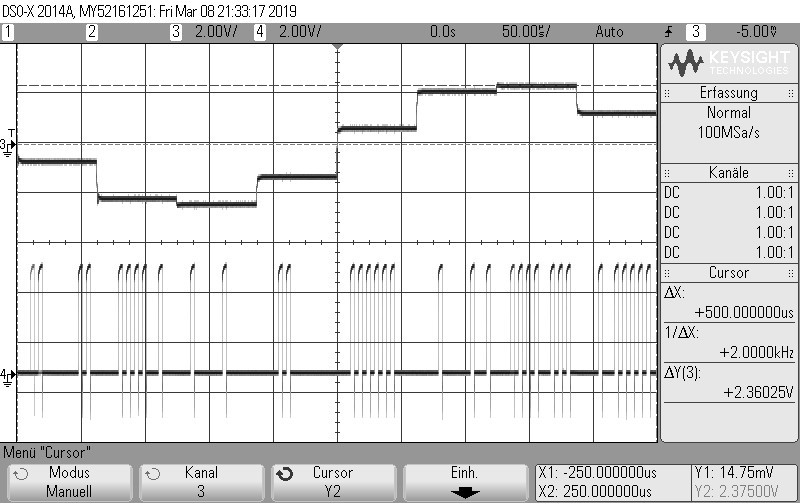
\includegraphics[width=1\textwidth]{scope_26}
         \caption{U\textsubscript{Puls-Code-Modulation} ist die unterste Spnnung}
   
          \label{fig:scope_26}
    \end{minipage}
    \end{figure}\\
    \newpage
    Fragen:\\
    1. Mit welcher Abtastfrequenz wird das Informationssignal abgetastet?\\
    Es wird mit 2kHz abgetastet.\\
    2. Stimmt das codierte PCM-Signal mit der Spannung U\textsubscript{S/H} zeitlich überein?\\
    Sie stimmen nicht überein, die Übertragung beginnt erst später, wie bei Abb. \ref{fig:scope_28} zu sehen ist.
    \begin{figure}[htbp]
    \begin{minipage}{1\textwidth}
         \centering
         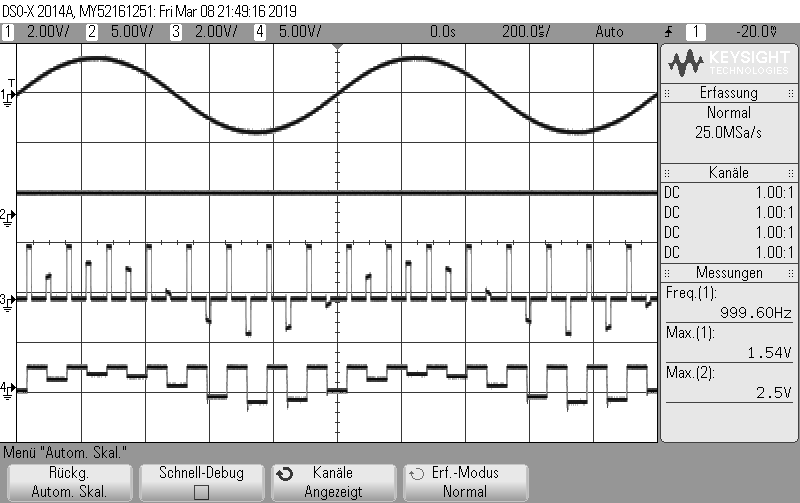
\includegraphics[width=1\textwidth]{scope_28}
         \caption{U\textsubscript{S}, U\textsubscript{PAM} und U\textsubscript{S/H}}
   
          \label{fig:scope_28}
    \end{minipage}
    \end{figure}\\
    \newpage
    3. In welcher Reihenfolge werden die Bits gesendet (zuerst MSB oder LSB)?\\
    Zuerst LSB, siehe Abb. \ref{fig:scope_27}
     \begin{figure}[htbp]
    \begin{minipage}{1\textwidth}
         \centering
         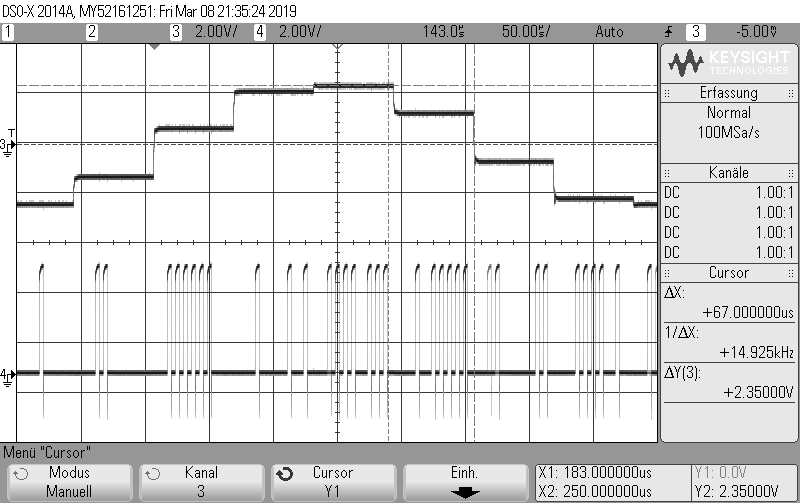
\includegraphics[width=1\textwidth]{scope_27}
         \caption{Digital, und Analogwert des Signals}
   
          \label{fig:scope_27}
    \end{minipage}
    \end{figure}
    \newpage
    .
    \end{document}

    
